%%%%%%%%%%%%%%%%%%%%%%%%%%%%%% -*- Mode: Latex -*- %%%%%%%%%%%%%%%%%%%%%%%%%%%%
%% 04-14.tex -- Managing Software Quality Using Hackystat
%% Author          : Aaron A. Kagawa
%% Created On  : Thu Sept 21 10:00:56 2004
%% Last Modified By: Aaron Kagawa
%% Last Modified On: Tue Sep 21 18:13:21 2004
%% Status          : Unknown
%% RCS: $Id: thesis.tex,v 1.3 2000/03/17 21:32:00 rbrewer Exp $
%%%%%%%%%%%%%%%%%%%%%%%%%%%%%%%%%%%%%%%%%%%%%%%%%%%%%%%%%%%%%%%%%%%%%%%%%%%%%%%
%%   Copyright (C) 1998 Robert Brewer
%%%%%%%%%%%%%%%%%%%%%%%%%%%%%%%%%%%%%%%%%%%%%%%%%%%%%%%%%%%%%%%%%%%%%%%%%%%%%%%
%% 
%% New LaTeX2e
\documentclass[11pt,proposal,times,thesis,actual]{uhthesis2e}
% substitute ``final'' for ``proposal'' to get actual thesis.

\usepackage[final]{graphicx}  %% New LaTeX2e graphics support
\usepackage{url}              %% Allows decent linebreaking of URLs
\usepackage{shapepar}         %% Makes shaped paragraphs
\usepackage{alltt}            %% A verbatim-like environment which allows font changes
\usepackage{rotating}         %% Allows text rotation
%%\usepackage{sideways}       %% Allows for turning pictures 90-degrees counter-clockwise
\usepackage{textcomp}         %% Allows for trademark symbol

\begin{document}
\title{Managing Software Quality Using Hackystat}
\author{Aaron A. Kagawa}
\degreemonth{May}
\degreeyear{2005}
\degree{Masters}
\chair{Philip M. Johnson}
\othermembers{...}
\numberofmembers{5}
\field{Information and Computer Sciences}
\versionnum{1.1.0}            %% Only printed in proposal mode

\maketitle

\begin{frontmatter}
%%\signaturepage 
%%\copyrightpage
%%%%%%%%%%%%%%%%%%%%%%%%%%%%%%%% -*- Mode: Latex -*- %%%%%%%%%%%%%%%%%%%%%%%%%%%%
%% 04-14-dedication.tex -- 
%% Author          : Aaron A. Kagawa
%% Created On      : Tue Sept 21 14:33:09 2004
%% Last Modified By: Aaron Kagawa
%% Last Modified On: Tue Sep 21 17:49:29 2004
%% RCS: $Id: 04-dedication.tex,v 1.3 2000/03/17 21:26:34 rbrewer Exp $
%%%%%%%%%%%%%%%%%%%%%%%%%%%%%%%%%%%%%%%%%%%%%%%%%%%%%%%%%%%%%%%%%%%%%%%%%%%%%%%
%%   Copyright (C) 1998 Robert Brewer
%%%%%%%%%%%%%%%%%%%%%%%%%%%%%%%%%%%%%%%%%%%%%%%%%%%%%%%%%%%%%%%%%%%%%%%%%%%%%%%
%% 

\begin{center}
To my family.
\end{center}

%%%%%%%%%%%%%%%%%%%%%%%%%%%%%%%% -*- Mode: Latex -*- %%%%%%%%%%%%%%%%%%%%%%%%%%%%
%% 04-14-acknowledgments.tex -- 
%% Author          : Aaron A. Kagawa
%% Created On      : Tue Sep 21 14:35:00 2004
%% Last Modified By: Aaron Kagawa
%% Last Modified On: Tue Sep 21 17:48:57 2004
%% RCS: $Id: 04-acknowledgments.tex,v 1.3 2000/03/17 21:26:58 rbrewer Exp $
%%%%%%%%%%%%%%%%%%%%%%%%%%%%%%%%%%%%%%%%%%%%%%%%%%%%%%%%%%%%%%%%%%%%%%%%%%%%%%%
%%   Copyright (C) 1998 Robert Brewer
%%%%%%%%%%%%%%%%%%%%%%%%%%%%%%%%%%%%%%%%%%%%%%%%%%%%%%%%%%%%%%%%%%%%%%%%%%%%%%%
%% 

\begin{acknowledgments}
This research would not be possible without the following people who have
provided me with guidance, support, and encouragement along the way.

The Collaborative Software Development Laboratory Staff; Dr. Philip Johnson, Hongbing
Kou, Qin Zhang, Michael Paulding, Takuya Yamashita, Burt Leung, and Melissa 
Rota. 

My thesis committe members;

And last of all, my family.

\end{acknowledgments}
% LocalWords:  tex Sep Exp Agustin
% LocalWords:  CSDL Philip Staver Albritton Jitender Miglani
% LocalWords:  Hongbing Kou Kagawa Chan Takuya Yamashita Peterson Crosby

%%%%%%%%%%%%%%%%%%%%%%%%%%%%%% -*- Mode: Latex -*- %%%%%%%%%%%%%%%%%%%%%%%%%%%%
%% 04-14-abstract.tex -- Thesis white paper - software inspections
%% Author          : Aaron A. Kagawa
%% Created On      : Mon Sep 23 11:52:28 2004
%% Last Modified By: Aaron Kagawa
%% Last Modified On: Fri Feb  4 16:07:06 2005
%% RCS: $Id$
%%%%%%%%%%%%%%%%%%%%%%%%%%%%%%%%%%%%%%%%%%%%%%%%%%%%%%%%%%%%%%%%%%%%%%%%%%%%%%
%%   Copyright (C) 2004 Aaron A. Kagawa
%%%%%%%%%%%%%%%%%%%%%%%%%%%%%%%%%%%%%%%%%%%%%%%%%%%%%%%%%%%%%%%%%%%%%%%%%%%%%%%
%% 

\begin{abstract}  % 200 words
Imagine that your project manager has budgeted 200 person-hours for the
next month to inspect newly created source code. Unfortunately, in order
to inspect all of the documents adequately, you estimate that it will
take 400 person-hours. However, your manager refuses to increase the
budgeted resources for the inspections. How do you decide which documents
to inspect and which documents to skip?

The classic definition of inspection does not provide any advice on how to
handle this situation. For example, the notion of entry criteria used in
Software Inspection \cite{Gilb93} determines when documents are ready for
inspection rather than if inspection is needed at all \cite{Ebenau94}.

%% I could talk about previous approaches here. Sampling and Up-Stream documents

This research will investigate how to prioritize inspection resources and
apply them to areas of the system that need them more. It is commonly
assumed that defects are not uniformly distributed across all documents in
a system - a relatively small subset of a system accounts for a relatively
large proportion of defects \cite{Boehm01}.  If inspection resources are
limited, then it will be more effective to identify and inspect the
defect-prone areas.

To accomplish this research, I will construct a framework based upon
automated process and product measures to distinguish documents that are
``more in need of inspection'' (MINI) from those ``less in need of
inspection'' (LINI). Some of the process and product measures include:
reported defects, unit tests, test coverage, active time, and number of
changes. Based on this framework, I hypothesize that the inspection of MINI
documents will generate more critical defects than LINI documents.

%% Each measure acts as an independent variable for determining the inspection
%% candidacy of a document and can be assigned an individual weight. 
%%Each measure affects the determination of ``more and less'' differently.
%%For example, suppose that test coverage should be weighted more than active
%%time. Therefore, weights of each measure will be calibrated based on my
%%initial guesses.  

My research will employ a very simple evaluation strategy, which includes
inspecting MINI and LINI software code and checking to see if MINI code
inspections generate more defects than LINI code inspections. There are
three milestones that measure my progress in this research. Milestone 1:
Implementation of Hackystat Extension, January 2005. Milestone 2: Completed
evaluation, March 2005. Milestone 3: Thesis submission and defense, May
2005.

\end{abstract}






%%\tableofcontents
%%\listoftables
%%\listoffigures
\end{frontmatter}

%%%%%%%%%%%%%%%%%%%%%%%%%%%%%% -*- Mode: Latex -*- %%%%%%%%%%%%%%%%%%%%%%%%%%%%
%% 04-14-ch1.tex -- 
%% Author          : Aaron A. Kagawa
%% Created On      : Tue Sept 21 09:43:42 2004
%% Last Modified By: Aaron Kagawa
%% Last Modified On: Thu Sep 23 23:17:43 2004
%% Status          : Unknown
%% RCS: $Id: thesis-abstract.tex,v 1.1 1998/09/19 01:24:42 jagustin Exp $
%%%%%%%%%%%%%%%%%%%%%%%%%%%%%%%%%%%%%%%%%%%%%%%%%%%%%%%%%%%%%%%%%%%%%%%%%%%%%%%
%%   Copyright (C) 1995 University of Hawaii
%%%%%%%%%%%%%%%%%%%%%%%%%%%%%%%%%%%%%%%%%%%%%%%%%%%%%%%%%%%%%%%%%%%%%%%%%%%%%%%
%% 


\chapter{Introduction}
Provide an introduction to whole thesis.

This chapter will introduce you to the main ideas of this thesis. We will
first briefly look at what sofware quality is and the problems that is
associated with trying to achieve high software quality. Next, I will
introduce Hackystat and the Hackystat extension that I will be building to
help address some of the problems associated with managing software quality.


\section{Software Quality has Many Meanings}

The term ``Software Quality'' has many meanings. This is a test citation \cite{humphrey85}.

\begin{description}
\item Attributes:
\begin{enumerate}
\item The degree to which software possesses a desired combination of attributes
\cite{ieee-glossary83}.
\item The composite of all attributes which describe the degree of
excellence of the computer system \cite{fisher79}.
\item The degree to which a software product possesses a specified set of
attributes necessary to fulfill a stated purpose \cite{reifer85}.
\item Quality is a collection of attributes: portability, reliability,
efficiency, usability, testability, understandibility, and modifiability  \cite{glass79}
\end{enumerate}
\item Others
\begin{enumerate}
\item The fitness for use of the total software product \cite{schulmeyer87}
\end{enumerate}
\end{description}

And there is more. People affect quality. 

Whatever the definition, developers and managers alike need to strive for
the very highest of quality in every project they do. However, if people
cannot agree on what quality is then how are they to improve it? When the
very definition of something is faulty anything built upon that will very
likely be faulty as well. This is the bane of any quality assurance
program. 

This isn't to say that there have been 

\section{Quality is a Subjective Term}
Software Quality has many different meanings because it is subjectively
interpreted differently. Like all subjective terms, Software quality means
different things to different people.  Attempts in the software engineering
community to use qunatifiable measures of quality is useful until the exact
meaning of quality is challenged by others holding there own subjective
meaning. Here lies the extraordinary problem with acheiving high software
quality that is recognized by our peers.

In other engineering fields, like Mechanical Engineering, it is much easier
to view quality as a qualitative term because the products produced by
other fields are physical objects that can be tested. Software on the other
hand, is not physical, it can not be picked up and banged against the
ground to determine quality. It isn't made up of physical materials like
metal. Metal has universally accepted quanitifiable measures and
theoritical laws that apply to it. A product that is created with metal
thus has the quantifiable measures associated with the material itself.
Attempts to fully quanitify software quality will always fail unless it can
be constructed with ``materials'' that have fully quantifiable measures and
are universally accepted.

Quality of software is much like evaluating the quality of a cup of coffee.
It depends on subjective measures, for example, the aroma of the coffee
grinds. We can subjectively sense the differences of a gourmet cup of
coffee from those we find in our hotel room. The exact process of that
determination is very debatable and is the essence of a subjective measure.

However, subjective measures, like software quality, need not be based
soley on our own intuition. As in determining the quality of a coffee grind, 
we can base our decissions on quantitative data. For example, the price of
a coffee grind provides a quantifiable measure on which we base our
subjective view. This isn't to say that the price accurately reflects the
``quality'' of a coffee grind but from our experiences we assume it to be true.

Why attempt to quantify the un-quantifiable? Why try to quanitify the
quality of coffee when we already have a good understanding of how good a
cup of coffee is using our own subjectivity? Until someone invents a universally
acceptable quantifiable measure of a subjective meaing, we should embrace its
existance instead of ignoring it. As I previously stated, it isn't the case 
that quantifiable measures of other aspects of a product is invalid. We
should use these measures to form our subjective view of quality.

In this thesis I will attempt to use quantifiable measures of software to
determine subjective quality. The important distiction between previous
works in this field is that subjectivity will be modeled into the quality
measure itself.


\section{Some Software Quality Measures}
This section provides some software quality measures that are in use.

Defect Density

\section{The Hackystat Quality Extension: A system to manage the quality of a
project}
As I previously stated subjectivity is a major part of how people view
software quality. Different organiziations have view quality in different
ways and more importantly this should be accepted and embraced. Simply
ignoring subjectivity will cause the age old complaint by developers and
managers, ``I don't care about quality''. It is important to realize that
everyone cares about making a good product but they simply don't agree with 
the definitions that others give quality.


\section{Thesis Statement}
This research investigates the 



















%%\include{04-14-ch2}
%%%%%%%%%%%%%%%%%%%%%%%%%%%%%%%% -*- Mode: Latex -*- %%%%%%%%%%%%%%%%%%%%%%%%%%%%
%% 04-14-appendix.tex -- 
%% Author          : Aaron A. Kagawa
%% Created On      : Tue Sept 21 12:04:50 2004
%% Last Modified By: Aaron Kagawa
%% Last Modified On: Tue Dec  7 23:01:04 2004
%% Status          : Unknown
%% RCS: $Id: 04-appendix.tex,v 1.3 2000/03/17 21:28:36 rbrewer Exp $
%%%%%%%%%%%%%%%%%%%%%%%%%%%%%%%%%%%%%%%%%%%%%%%%%%%%%%%%%%%%%%%%%%%%%%%%%%%%%%%
%%   Copyright (C) 1998 Robert Brewer
%%%%%%%%%%%%%%%%%%%%%%%%%%%%%%%%%%%%%%%%%%%%%%%%%%%%%%%%%%%%%%%%%%%%%%%%%%%%%%%
%% 

\appendix

\chapter{Consent Form}
\label{appendix:consent}
\begin{figure}[htbp]
  \centering
  \includegraphics[width=1.0\textwidth]{figs/ConsentForm_shrunk.eps}
  \caption{Consent Form}
  \label{fig:consent}
\end{figure}

\chapter{Questionnaires}
\label{appendix:questionnaire}

\begin{figure}[htbp]
  \centering
  \includegraphics[width=1.0\textwidth]{figs/hackyTelemetry-questionnaire-shrunk_1.eps}
  \caption{Questionnaire - Part 1}
  \label{fig:questionnaire1}
\end{figure}

\begin{figure}[htbp]
  \centering
  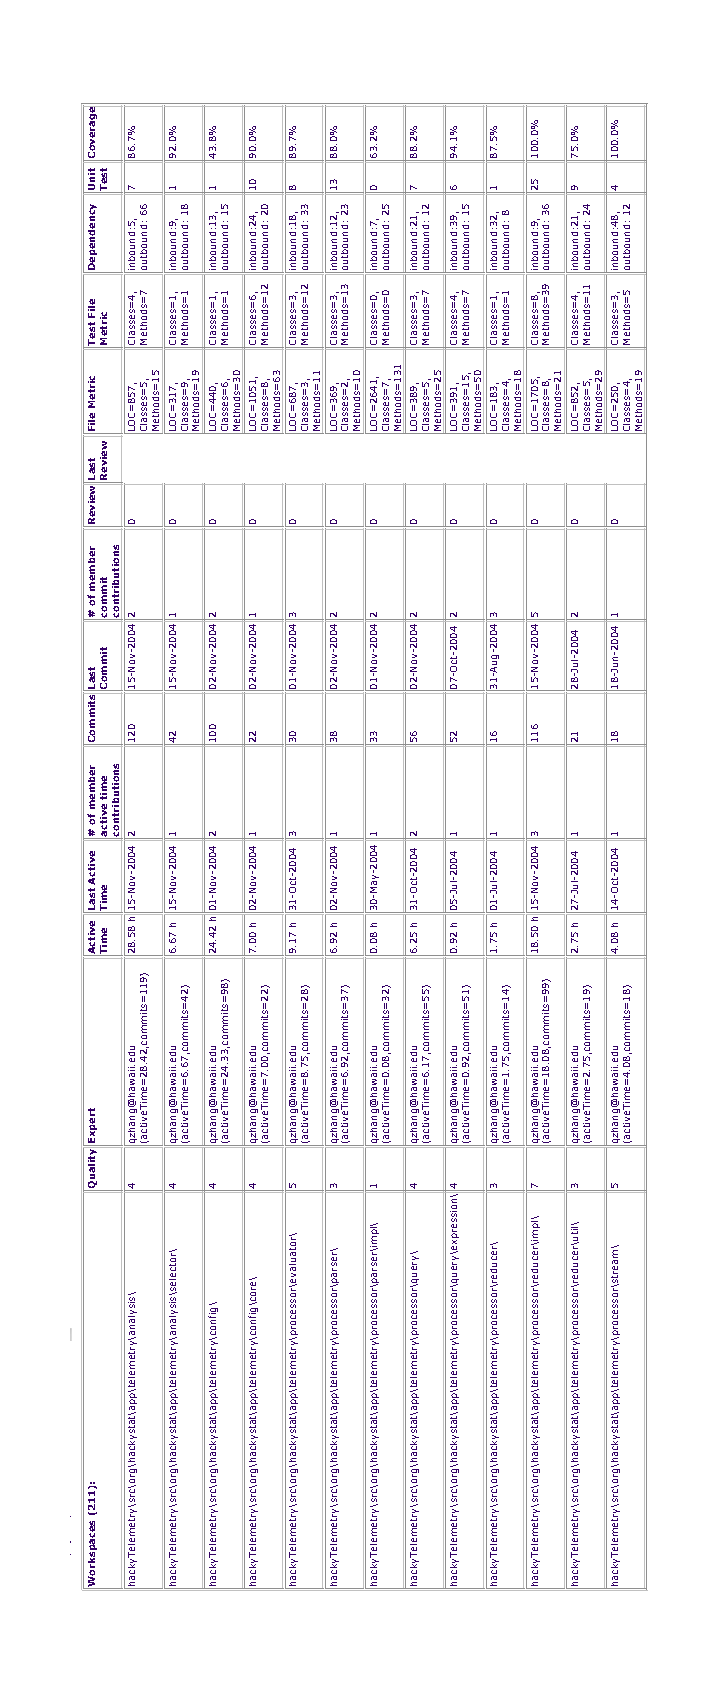
\includegraphics[width=0.63\textwidth]{figs/2004-11-18-hackyTelemetry.eps}
  \caption{Questionnaire - Part 2.1}
  \label{fig:questionnaire2.1}
\end{figure}

\begin{figure}[htbp]
  \centering
  \includegraphics[width=1.0\textwidth]{figs/hackyTelemetry-questionnaire-shrunk_2.eps}
  \caption{Questionnaire - Part 2.2}
  \label{fig:questionnaire2.2}
\end{figure}


\chapter{Inpsection Log and Results}
\label{appendix:log}
This appendix provides a journal of my processes throughout the evaluation
of Priority Ranked Inspection (PRI). I include several details about each
inspection that is conducted, which include: the PRI determination, some of 
the measures that PRI used to create the determination, my subjective
opinions about the package to be inspected, the results in terms of the
number of issues found and their severity, and my subjective opinions on
the PRI determination given the results.

Using this journal, I hope to construct a general guidelines for the use of
and calibration of PRI for other organizations and projects.

%\begin{figure}[htbp]
%  \centerline{\psfig{figure=figs/Acceptance.ps}}
%  \caption{Acceptance}
%  \label{fig:acceptance}
%\end{figure}

\begin{figure}[htbp]
  \centering
  \includegraphics[width=1.0\textwidth]{figs/engineeringlog_word_html_1.eps}
  \caption{Inspection Log and Results - Part 1}
  \label{fig:log1}
\end{figure}

\begin{figure}[htbp]
  \centering
  \includegraphics[width=1.0\textwidth]{figs/engineeringlog_word_html_2.eps}
  \caption{Inspection Log and Results - Part 2}
  \label{fig:log2}
\end{figure}

\begin{figure}[htbp]
  \centering
  \includegraphics[width=1.0\textwidth]{figs/engineeringlog_word_html_3.eps}
  \caption{Inspection Log and Results - Part 3}
  \label{fig:log3}
\end{figure}

\begin{figure}[htbp]
  \centering
  \includegraphics[width=1.0\textwidth]{figs/engineeringlog_word_html_4.eps}
  \caption{Inspection Log and Results - Part 4}
  \label{fig:log4}
\end{figure}

\begin{figure}[htbp]
  \centering
  \includegraphics[width=1.0\textwidth]{figs/engineeringlog_word_html_5.eps}
  \caption{Inspection Log and Results - Part 5}
  \label{fig:log5}
\end{figure}

\begin{figure}[htbp]
  \centering
  \includegraphics[width=1.0\textwidth]{figs/engineeringlog_word_html_6.eps}
  \caption{Inspection Log and Results - Part 6}
  \label{fig:log6}
\end{figure}

\begin{figure}[htbp]
  \centering
  \includegraphics[width=1.0\textwidth]{figs/engineeringlog_word_html_7.eps}
  \caption{Inspection Log and Results - Part 7}
  \label{fig:log7}
\end{figure}

\begin{figure}[htbp]
  \centering
  \includegraphics[width=1.0\textwidth]{figs/engineeringlog_word_html_8.eps}
  \caption{Inspection Log and Results - Part 8}
  \label{fig:log8}
\end{figure}

\begin{figure}[htbp]
  \centering
  \includegraphics[width=1.0\textwidth]{figs/engineeringlog_word_html_9.eps}
  \caption{Inspection Log and Results - Part 9}
  \label{fig:log9}
\end{figure}







\bibliography{/export/home/csdl/bib/quality, /export/home/csdl/bib/csdl-trs}
\bibliographystyle{plain}
\end{document}






























